Este capítulo apresenta um estudo exploratório realizado com o objetivo de verificar a viabilidade e aperfeiçoar a proposta com base nas descobertas e desafios enfrentados durante o processo. Destaca-se que este estudo teve o foco apenas na análise das avaliações de acessibilidade e não explorou as sugestões de modificações e as alterações realizadas no código das aplicações. Todas as decisões de projeto e metodologia adotada estão em conformidade com o que foi descrito no Capítulo~\ref{chap:proposta}.
Além disso, também são descritas as atividades já realizadas do cronograma proposto.

\section{Questões de pesquisa}

As seguintes questões de pesquisa foram definidas para este estudo exploratório:
\begin{itemize}
 \item RQ1 - Quantas avaliações de usuário são relacionadas a acessibilidade e qual é a sua distribuição? 
 \item RQ2 - Qual é a diversidade de tópicos de acessibilidade abordados nas avaliações dos usuários?
 \item RQ3 - Quais são as notas associadas às avaliações que abordam aspectos de acessibilidade?  
\end{itemize}

\section{Seleção de aplicativos móveis}

Os critérios de seleção dos aplicativos para este estudo seguem os critérios definidos na Seção~\ref{sec:selecao}. Portanto, foram selecionadas aplicações da plataforma Android que satisfaziam as seguintes condições: estavam disponíveis na Google Play Store e o código-fonte estava armazenado em um repositório público da plataforma GitHub. Ao todo, apenas 701 aplicativos dentre os mais de 2000  indexados no FDroid\footnote{Dados de julho/2019} satisfizeram esses critérios.

A Tabela~\ref{tab:summarygps} mostra a distribuição de alguns atributos dos aplicativos selecionados por meio de estatística descritiva utilizando o resumo dos cinco números (mínimo amostral, quartil inferior, 
mediana, quartil superior, máximo amostral), a média e o desvio padrão. 
A maioria dos aplicativos tem até 9 atividades, mas há aplicativos muito maiores, como o ``Slide for Reddit'', por exemplo, que possui 91 atividades.

\begin{table}[htb]
%\setlength{\tabcolsep}{0pt}

\centering
\caption{Statistics on the Google Play Store sample}
\small
\label{tab:summarygps}
\begin{tabular}{lrrrrr}
\hline
             & Atividades & Nota & Avaliações     & Instalações  & Comentários \\
\hline
Mínimo          & 1          & 0     & 0            & 0         & 0       \\
Quartil Inferior           & 2          & 4           & 50    & 1K      & 4       \\
Mediana       & 5          & 4.3   & 130         & 10K     & 22      \\
Quartil Superior          & 9          & 4.6   & 836        & 50K     & 145     \\
Máximo          & 92         & 5     & 3.6M    & 100M & 4480    \\
Média         & 8.16       & 4.16  & 12.4K     & 550K+    & 305.4   \\
Desvio Padrão        & 10.5       & 0.79  & 151.6K  & 5.7M   & 840.8  \\
\hline
\end{tabular}
\end{table}

A maioria dos aplicativos possui uma boa nota e a maioria foi avaliada por até 836 usuários. O número de avaliações apresentado na tabela é diferente do número de comentários, pois quando um usuário faz uma avaliação ele é obrigado a atribuir uma nota, mas não é obrigado a inserir um comentário. Existem aplicativos que possuem um número muito alto de avaliações, como o Telegram, que possui 3,6 milhões de avaliações. O Telegram também é o aplicativo mais instalado (100 milhoes de istalações).
Por outro lado, o número de comentários não é muito alto, pois a maioria dos aplicativos recebeu até no máxmio 145 comentários em suas avaliações. O número máximo de revisões desta amostra é de 4480 em razão das limitações da API utilizada. Esta limitação não teve muito impacto neste estudo exploratório porque apenas 15 aplicativos (2\%) possuem mais de 4480 revisões registradas na Google Play Store.


\section{Extração e seleção das avaliações}

Uma aplicação escrita na linguagem Python foi escrita para consumir os dados da Google Play Store utilizando a API \emph{google-play-api}\footnote{https://github.com/facundoolano/google-play-api}. Como mencionado anteriormente, na versão utilizada, esta API só permite o retorno de no máximo 4480 avaliações de cada aplicativo. Além disso, só foram recuperadas avaliações escritas em inglês, que é o idioma padrão definido pela API.


A seleção das avaliações que possivelmente estão relacionadas a algum aspecto de acessibilidade da aplicação foi feita por meio da utilização de palavras-chave aplicadas aos comentários dos usuários. 
Para isso, um conjunto de palavras-chave foi definido com base nas diretrizes de acessibilidade da BBC~\cite{bbc}. Este guia de acessibilidade possui 54 recomendações que são classificadas em onze diferentes categorias: áudio e vídeo (5); design (12); editorial (3); foco (6); formulários (6); imagens (2); links (3); notificações (4); scripts e conteúdo dinâmico (4); estrutura (4); e texto equivalente (5). 
Este padrão foi selecionado porque ele tem o foco em aplicações móveis e possui exemplos de implementação e de teste de cada recomendação, o que permite compreender melhor os tipos de problemas de acessibilidade tratados no guia. 

Foram definidas 213 palavras-chave com base na análise de cada recomendação do guia. 
A Tabela~{tab:keywords} mostra exemplos das palalavras-chave utilizadas.
Note que foram utilizadas variantes das palavras (exemplo: \textit{cannot see} e \textit{can't see}, ou \textit{color} e \textit{colour}, ou \textit{impaired} e \textit{impairement}) para garantir que nenhuma avaliação relevante fosse excluída. Infelizmente, não é possível capturar casos em que as palavras foram escritas com a grafia errada. A lista completa das palavras-chave podem ser vistas em um repositório criado para armazenar dos dados deste estudo\footnote{https://github.com/marceloeler/data-ihc2019}.


\begin{table}[!htb]
\small
\caption{Exemplos de palavras-chave utilizadas para selecionar avaliações relacionadas à acessibilidade das aplicações}
\label{tab:keywords}
\begin{tabular}{|l|l|}
\hline
Categorias & Palavras-chave \\
\hline
Gerais                    & accessibility, disability, screen reader, Talkback, operable, impaired, 
\\& impairment                                               \\

\hline
Áudio/Vídeo             & subtitle, sign language, audio description,
 transcript, autoplay, mute, \\& volume                                                 \\

\hline
Design                      & contrast, background color, blind, flicker,
 visual cue, touch size, \\&overlap, font size, 
 dark/light mode, eyestrain, seizure, can't see \\

\hline
Editorial                   & consist. label, language, visual/audio cue                                                                \\

\hline
Foco                       & focusable, control focus, keyboard trap, 
 focus order, navigable                        \\

\hline
Formulários                       & unique label, missing label, content description,
 input type, \\& input format, focusable                                                                        \\

\hline
Imagens                      & image of text, hidden text, text alternative,
background image                                                                                               \\

\hline
Links                       & link description, unique desc., duplicate
link, alternative format \\

\hline
Notificações               & inclusive, haptic, vibration, feedback, alert 
 dialog, understandable, \\& unfamiliar                                                                             \\

\hline
Conteúdo dinâmico & animated content, page refresh, automatic  
refresh, timeout,  adaptable, \\&input sign                                                               \\

\hline
Estrutura                   & page title, screen title, heading, header                                                                                                         \\
\hline
Texto equivalente             & alternative text, non-visual, blind, screen reader, content description  \\
\hline
\end{tabular}
\end{table}

O uso de palavras-chave pode trazer muitos falsos positivos, uma vez que várias palavras utilizadas podem ter conotações diferentes em diferentes contextos. Por isso foi realizada uma análise manual de todas as avaliações que possuíam pelo menos uma palavra-chave definida. Neste estudo, apenas uma pessoa fez a análise manual das avaliações. Além disso, as avaliações não selecionadas por palavras-chave não foram analisadas para saber se alguma delas não foi selecionada pela ausência de alguma palavra-chave relevante e que não foi utilizada. Durante a análise manual, as avaliações confirmadas também foram classificadas em: 
requisições, quando o usuário reporta algum problema de acessibilidade ou solicita alguma modificação ou adição para tornar a aplicação mais acessível;
ou elogios, quando o usuário parabeniza o aplicativo pelo seu nível de acessibilidade.


\section{Análise dos resultados}

As avaliações selecionadas com base nas palavras-chave e na validação manual foram analisadas para responder as questões de pesquisa propostas no estudo exploratório. A seguir as respostas às questões de pesquisa são apresentadas em detalhes. 

 
\textbf{RQ1 - Quantas avaliações de usuário são relacionadas a acessibilidade e qual é a sua distribuição? }

No total, foram extraídas 214.053 avaliações completas (com nota e comentário) dos 701 aplicativos da amostra. 
Dessas avaliações, apenas 5.076 foram pré-selecionadas por meio das palavras-chave. 
Após a análise manual, o número de avaliações relacionadas à acessibilidade das aplicações foi reduzido para 2.663, o que representa apenas 1.24\% de todas as avaliações completas extraídas.

As avaliações de acessibilidade não estão igualmente distribuídas entre os aplicativos da amostra.
Só 40\% dos aplicativos (276) possuem pelo menos uma avaliação relacionada a acessibilidade.
É importante ressaltar que 92\% (197.419) de todas as avaliações extraídas foram realizadas para esses 276 aplicativos, indicando que quanto menos avaliações, menos as chances de haver uma avaliação de acessibilidade. 
De fato, a correlação de Spearman calculada entre o número de avaliações e o número de avaliações de acessibilidade é de 0.73, o que representa uma forte correlação.

As avaliações de acessibilidade não estão distribuídas igualmente entre os 276 aplicativos.
Quase 65\% das avaliações de acessibilidade (1.745) estão concentradas em apenas 35 aplicativos. 
Dentre esses 35 aplicativos, três possuem mais de 100 avaliações de acessibilidade enquanto os demais tem entre 19 e 79 avaliações cada. 
A Figura~\ref{fig:distributionreviewsapp} mostra a distribuição de avaliações de acessibilidade entre os aplicativos da amostra, com exceção dos 35 aplicativos mencionados anteriormente.
É possível perceber que a grande maioria de aplicativos tem menos do que nove avaliações de acessibilidade enquanto cerca de metade da amostra tem até três avaliações do tipo.


\begin{figure}[!htb]
\centering
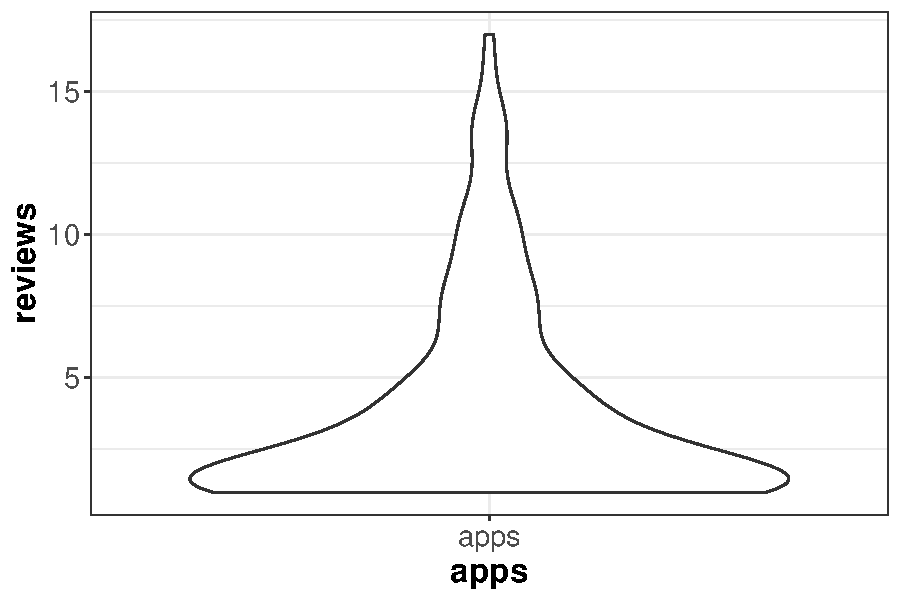
\includegraphics[scale=0.80]{imagens/distribution-accreviews-no-outlier-violin.pdf}
\caption{Distribuição das avaliações de acessibilidade entre os aplicativos da amostra}
\label{fig:distributionreviewsapp}
\end{figure}


A Figura~\ref{fig:distribution-proportion} mostra a distribuição da proporção entre as avaliações de acessibilidade e o número total de avaliações completas de cada aplicativo.
No geral, as avaliações de acessibilidade representam menos de 4\% de todas as reviões feitas para cada aplicativo. Para metade dos aplicativos, elas representam menos de 1.5\%.
Para uma pequena proporção de aplicativos, as avaliações de acessibilidade representam entre 4\% e 9\% das avaliações recebidas. Existem alguns aplicativos para os quais essa proporção varia entre 10\% e 16\%.
Há alguns casos em que o número de avaliações completas é tão pequeno que uma simples avaliação de acessibilidade representa uma grande proporção, como é o caso do aplicativo MuPDF mini, Booky McBookface, e GameDealz, cujas proporções são de 50\% (1/2), 40\% (2/5) e 33\% (1/3), respectivamente. 
\newline 

 \begin{figure}[!htb]
 \centering
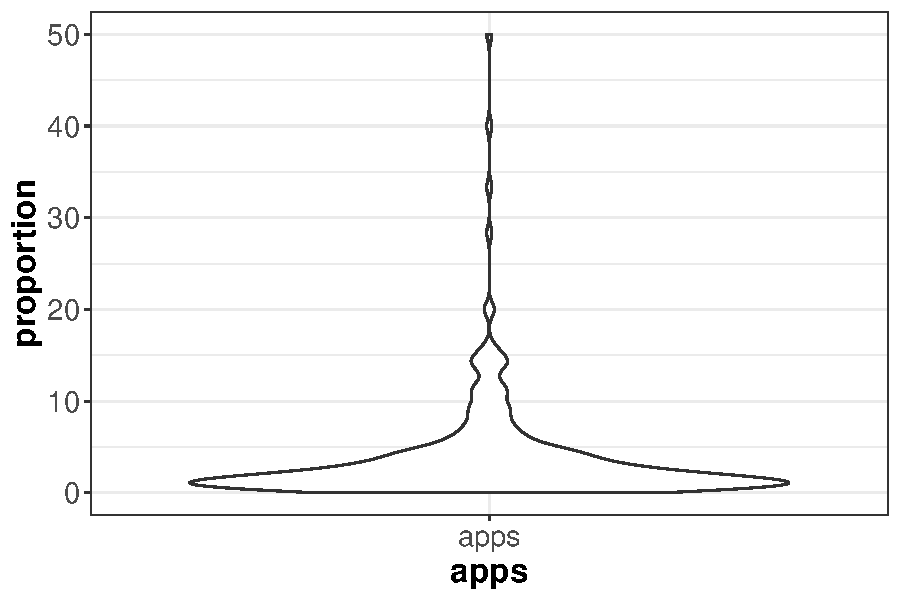
\includegraphics[scale=0.8]{imagens/distribution-proportion-accreviews}
\caption{Distribuição da proporção entre avaliações de acessibilidade e o total de avaliações de cada aplicativo}
\label{fig:distribution-proportion}
\end{figure}


\textbf{RQ2 - Qual é a diversidade de tópicos de acessibilidade abordados nas avaliações dos usuários?}

O objetivo desta questão de pesquisa é entender se os usuários abordam diferentes problemas de acessibilidade em suas avaliações ou se a maioria das avaliações tratam de um conjunto restrito de problemas. 
A Tabela~\ref{tab:keywords-reviews} mostra o número de avaliações de acessibilidade e aplicativos associado a cada palavra-chave utilizada para selecionar as avaliações. 
Nesta tabela só estão apresentadas as palavras-chave para as quais pelo menos uma avaliação estava associada. 

\begin{table*}[!htb]
\centering
\small
\setlength{\tabcolsep}{3pt}
\caption{Número de avaliações e aplicativos por palavra-chave}
\label{tab:keywords-reviews}
\begin{tabular}{lrr||lrr||lrr}
\hline
palavra          & avals. & apps & palavra          & avals. & apps &  palavra            & avals. & apps \\
\hline
dark mode        & 645     & 128  & metadata         & 20      & 12   & grouped            & 3       & 3    \\
zoom             & 491     & 80   & too bright       & 20      & 8    & seizures           & 3       & 1    \\
customization    & 309     & 50   & haptic           & 16      & 10   & select language    & 3       & 3    \\
font size        & 214     & 74   & scaling          & 16      & 11   & understandable     & 3       & 3    \\
volume           & 146     & 40   & control key      & 15      & 5    & vibration feedback & 3       & 3    \\
cannot see       & 128     & 57   & voice command    & 14      & 10   & actionable         & 2       & 1    \\
accessibility    & 74      & 44   & text-to-speech   & 13      & 9    & audio cue          & 2       & 2    \\
readable         & 72      & 47   & eyestrain        & 12      & 9    & missing label      & 2       & 2    \\
change font      & 68      & 44   & strain           & 12      & 9    & navigable          & 2       & 2    \\
hard to see      & 58      & 41   & backgrd. image & 11      & 8    & verbose            & 2       & 2    \\
backgrd. color   & 50      & 30   & screen reader    & 11      & 10   & captcha            & 2       & 2    \\
light mode       & 42      & 27   & change language  & 10      & 8    & audio description  & 1       & 1    \\
mute             & 42      & 25   & small widget     & 10      & 9    & container          & 1       & 1    \\
contrast         & 40      & 31   & stop button      & 10      & 5    & distinguishable    & 1       & 1    \\
subtitle         & 40      & 7    & impaired         & 9       & 9    & input type         & 1       & 1    \\
adjustable       & 34      & 23   & text reflow      & 9       & 3    & keyboard language  & 1       & 1    \\
blind            & 31      & 24   & timeout          & 9       & 7    & page refresh       & 1       & 1    \\
header           & 31      & 22   & consistency      & 7       & 7    & page title         & 1       & 1    \\
overlap          & 31      & 25   & epilepsy         & 7       & 1    & sign language      & 1       & 1    \\
pause button     & 27      & 17   & assistance       & 6       & 5    & svg image          & 1       & 1    \\
flicker          & 26      & 19   & colour coding    & 5       & 5    & switch device      & 1       & 1    \\
spacing          & 26      & 17   & transcript       & 5       & 5    & touch target       & 1       & 1    \\
migraine         & 25      & 3    & default language & 4       & 4    & adjust size        & 1       & 1    \\
input method     & 23      & 11   & older device     & 4       & 3    & adjust colour      & 1       & 1    \\
autoplay         & 21      & 17   & visual cue       & 4       & 4    &                    &         &     \\
\hline
\end{tabular}
\end{table*}

Claramente, as avaliações de acessibilidade estão concentradas em um pequeno conjunto de palavras-chave. Seis das palavras-chave mais populares são mencionadas em mais de 100 avaliações de diferentes aplicativos. Por exemplo, a palavra-chave \textit{dark mode} aparece em 628 avaliações de 128 aplicativos distintos, o que representa quase metade da amostra de aplicativos.

Como várias palavras-chave podem estar relacionadas a uma mesma diretriz ou princípio de acessibilidade (exemplo: \textit{dark mode}, \textit{night mode} e \textit{black mode}), 
as palavras-chave e as respectivas quantidades de avaliações foram agrupadas por tópicos (diretrizes, princípios ou temas) específicos de acessibilidade para facilitar a análise da diversidade de características abordadas.

A Tabela~\ref{tab:group-keywords} mostra, para cada tópico de acessibilidade (Coluna 1), o número de avaliações distintas (Coluna 2), a proporção das avaliações em relação às avaliações de acessibilidade (Coluna 3), o número de aplicativos distintos que tiveram uma avaliação relacionada (Coluna 4), e a proporção de aplicativos em relação aos aplicativos que possuem pelo menos uma avaliação (Coluna 5).
As diretrizes gerais da BBC não foram utilizadas para a organização dos tópicos apresentados na tabela porque eles são muito gerais e podem englobar muitas palavras-chave ao mesmo tempo.

\begin{table}[]
\centering
\caption{Distribuição de avaliações de acessibilidade e aplicativos por tópico de acessibilidade}
\label{tab:group-keywords}
\begin{tabular}{lrrrr}
\hline
Tópico         & Avals. & \% (Avals.) & Apps & \% (Apps) \\
\hline
Theme/Mode    & 726     & 27\%     & 144  & 52\%  \\
Zoom          & 506     & 19,0\%     & 83   & 30,1\%  \\
Customization & 351     & 13\%     & 63   & 23\%  \\
Media         & 309     & 11,6\%     & 82   & 29,7\%  \\
Font          & 249     & 9,4\%      & 83   & 30,1\%  \\
Contrast      & 218     & 8\%        & 91  & 33\%  \\
Impairment    & 135     & 5,1\%      & 70   & 25,4\%  \\
Flickering    & 87      & 3,3\%      & 31   & 11,2\%  \\
Accessibility & 74      & 2,8\%      & 44   & 15,9\%  \\
Size          & 66      & 2,5\%      & 45   & 16,3\%  \\
Input alternatives        & 54      & 2,0\%      & 25   & 9,1\%   \\
Feedback      & 19      & 0,7\%      & 11   & 4,0\%   \\
Language      & 15      & 0,6\%      & 11   & 4,0\%  \\
\hline
\end{tabular}
\end{table}

O tópico \textit{Theme/Mode} é o mais popular entre as avaliações uma vez que 27\% das avaliações de acessibilidade estão relacionadas a este tópico, e quase metade das aplicações tem este tipo de avaliação. 
Este tópico agrega todas as avaliações que mencionam modos de cores e temas das interfaces dos aplicativos. 
O segundo tópico mais popular é o relacionado a funcionalidades de \textit{zoom} (19\% das revisões de acessibilidade e 30\% das aplicações).
O terceiro tópico mais popular está relacionado à personalização do aplicativo, representando 13\% das revisões e relacionados a 23\% dos aplicativos. 
Diversos outros tópicos estão presentes em um número menor de avaliações de acessibilidade, mas muitos deles estão relacionados com um grande número de aplicativos. 

Além da análise de todas as avaliações em conjunto, também foram realizadas análises das diversidades de tópicos de acessibilidade de cada aplicativo isoladamente. 
Figure~\ref{fig:distributiontopicsapps} mostra a distribuição de palavras-chave encontradas nas avaliações de acessibilidade de cada aplicativo (lado esquerdo). 
No geral, há pouca diversidade de palavras-chave nas avaliações de cada aplicativo analisado individualmente. 
A correlação de Spearman entre a diversidade de palavras-chave e o número de avaliações em cada aplicativo é de 0.93, o que indica que a diversidade aumenta conforme aumenta o número de avaliações.


 \begin{figure}[!htb]
 \centering
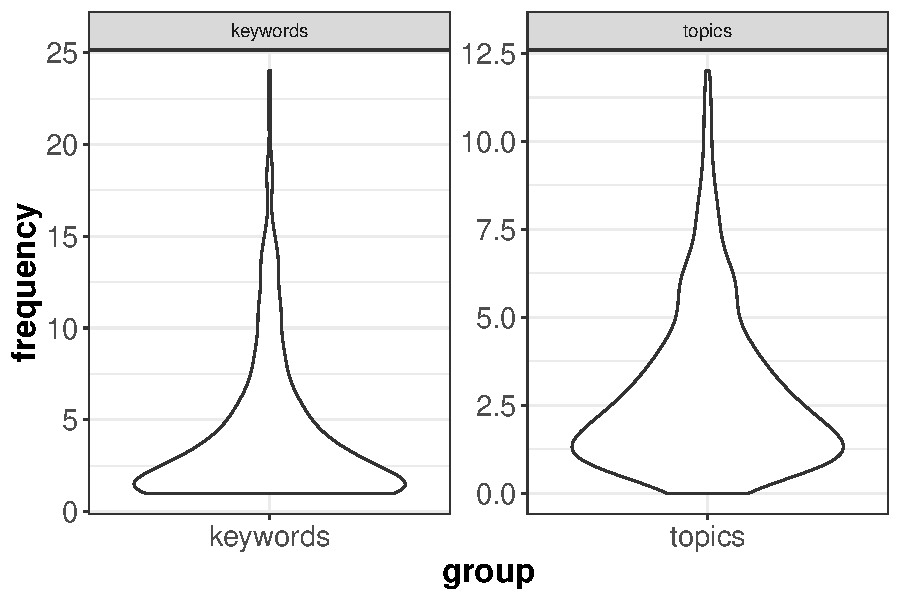
\includegraphics[scale=0.8]{imagens/distribution-topics-keywords.pdf}
\caption{Distribuição de tópicos de acessibilidade e palavras-chave nas avaliações de cada aplicativo}
\label{fig:distributiontopicsapps}
\end{figure}


Para a maioria dos aplicativos, as avaliações de acessibilidade estão relacionadas a no máximo seis palavras-chave. 
Para metade dos aplicativos, no máximo três palavras-chave são mencionadas. 
Poucos aplicativos tem avaliações que mencionam mais de 15 palavras-chave. 
Um dos aplicativos que foge ao padrão é o \textit{Cool Reader}, pois em suas avaliações foram encontradas 36 palavras-chave distintas. 


A diversidade de palavras-chave não é uma indicação de que diversos aspectos de acessibilidade são tratados uma vez que muitas delas estão relacionadas a um mesmo problema, e por isso uma análise por tópico deve ser realizada. 
A Tabela~\ref{fig:distributiontopicsapps} mostra a distribuição de tópicos de acessibilidade relacionados a cada avaliação de acessibilidade (lado direito). 
Note que as avaliações de acessibilidade para a maioria dos aplicativos estão concentradas em dois a quatro tópicos, enquanto alguns aplicativos possuem avaliações associadas a quase todos os tópicos abordados. 
O aplicativo \textit{Calculator}, por exemplo, tem avaliações de acessibilidade que abordam 12 tópicos de acessbilidade distintos. 
Embora a correlação de Spearman entre a diversidade de tópicos e o número de avaliações seja de 0.87, o que representa uma correlação forte, este aplicativo possui apenas 60 avaliações.


\textbf{RQ3 - Quais são as notas associadas às avaliações que abordam aspectos de acessibilidade?}


Not all reviews have features requests or bug reports. Many users give positive feedback on the apps they like. 
During our analysis, a review was marked as a compliment when a positive feedback was given on some accessibility aspect of the app. 
For instance, the review \textit{``I am totally blind - and Cool Mic is fully compatible with Android's built in TalkBack screenreader. Great work guys!''} is a positive feedback.
In our sample, around 76\% (2018) of the accessibility reviews are requests or complaints, and 24\% (645) are compliments. 
The 645 positive feedback on accessibility are distributed over 110 apps, while the requests/complaints reviews are distributed over 262 apps. There are 166 mobile apps that received only requests/complaints and 14 mobile apps that received only compliments.

One of the purposes of this research question is to find out whether users give a bad score when make a request related to accessibility and a good score when praise the app for its accessibility. 
\autoref{fig:reqcompscores} shows a violin plot to compare the scores obtained for these two samples. Surprisingly, it seems there is no significant difference between these two groups. 

 \begin{figure}[!htb]
 \centering
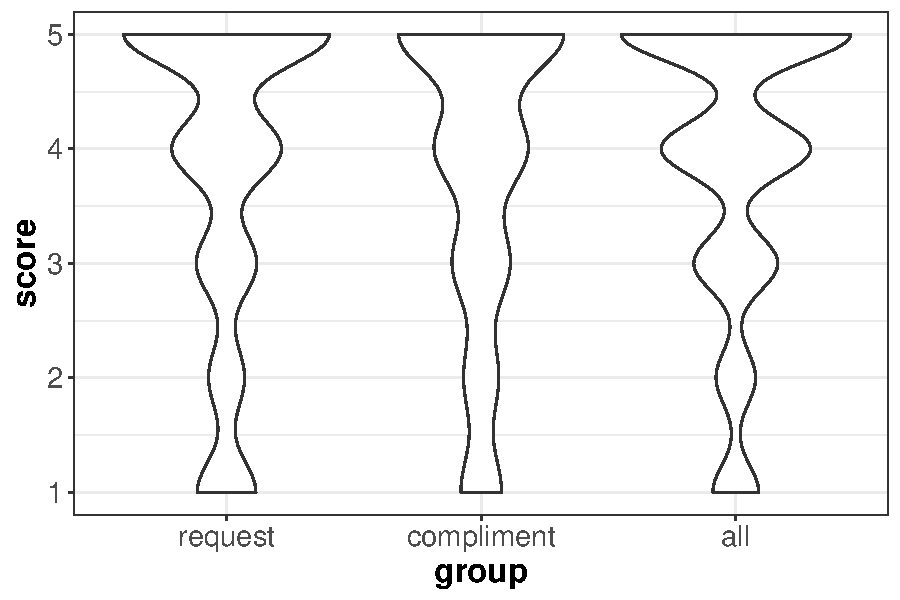
\includegraphics[scale=0.8]{imagens/scores-compliment-request.pdf}
\caption{Comparison between the scores associated with request and compliment reviews}
\label{fig:reqcompscores}
\end{figure}

In addition, we want to know whether reviews associated with different topics or keywords present lower or greater scores. 
\autoref{fig:scoresthemes} shows a violin plot to compare the scores of reviews related to specific accessibility topics (cf. \autoref{tab:group-keywords}). In this case, we only plotted data from reviews that contain accessibility requests or complaints. For some accessibility topics, even though users requested features that can make the mobile app more accessible, scores are concentrated in 4 or 5. This is the case of topics such as, for example, ``customization'', ``font'', ``media'', ``size'' and ``theme''. For other topics, it is clear that the reviews scores are concentrated between 2 and 4. The concentration of scores below 3 related to the keywords ``contrast'', ``flickering'' and ``zoom'' indicates that users are more affect by those issues than others.

 \begin{figure*}[!htb]
 \centering
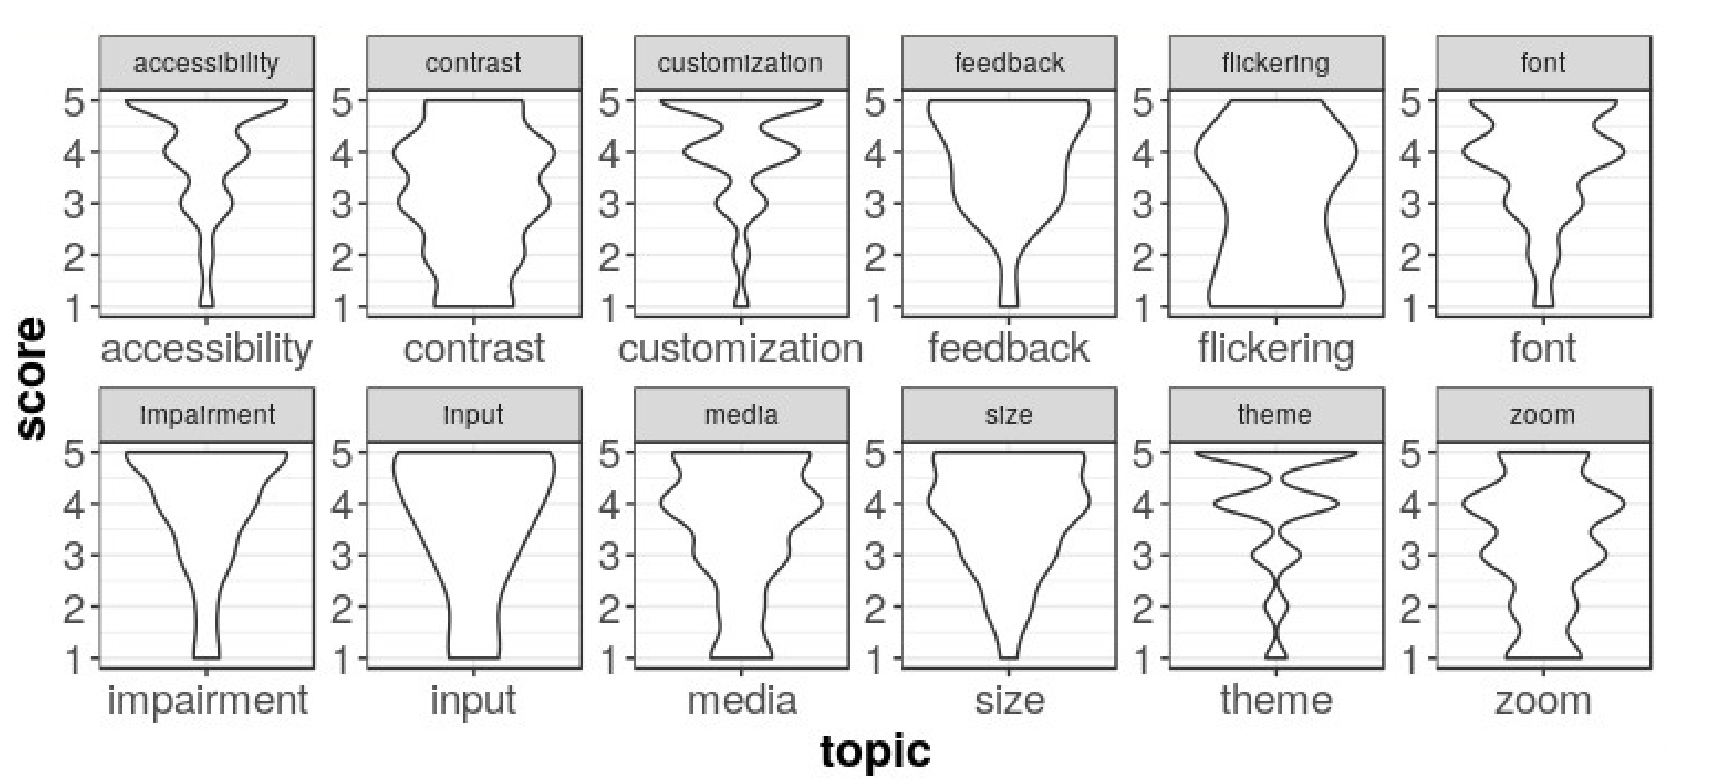
\includegraphics[scale=0.57]{imagens/score-themes-adapt.pdf}
\caption{Scores associated with the reviews that address an accessibility topic (cf. \autoref{tab:group-keywords})}
\label{fig:scoresthemes}
\end{figure*}

 \begin{figure*}[!htb]
 \centering
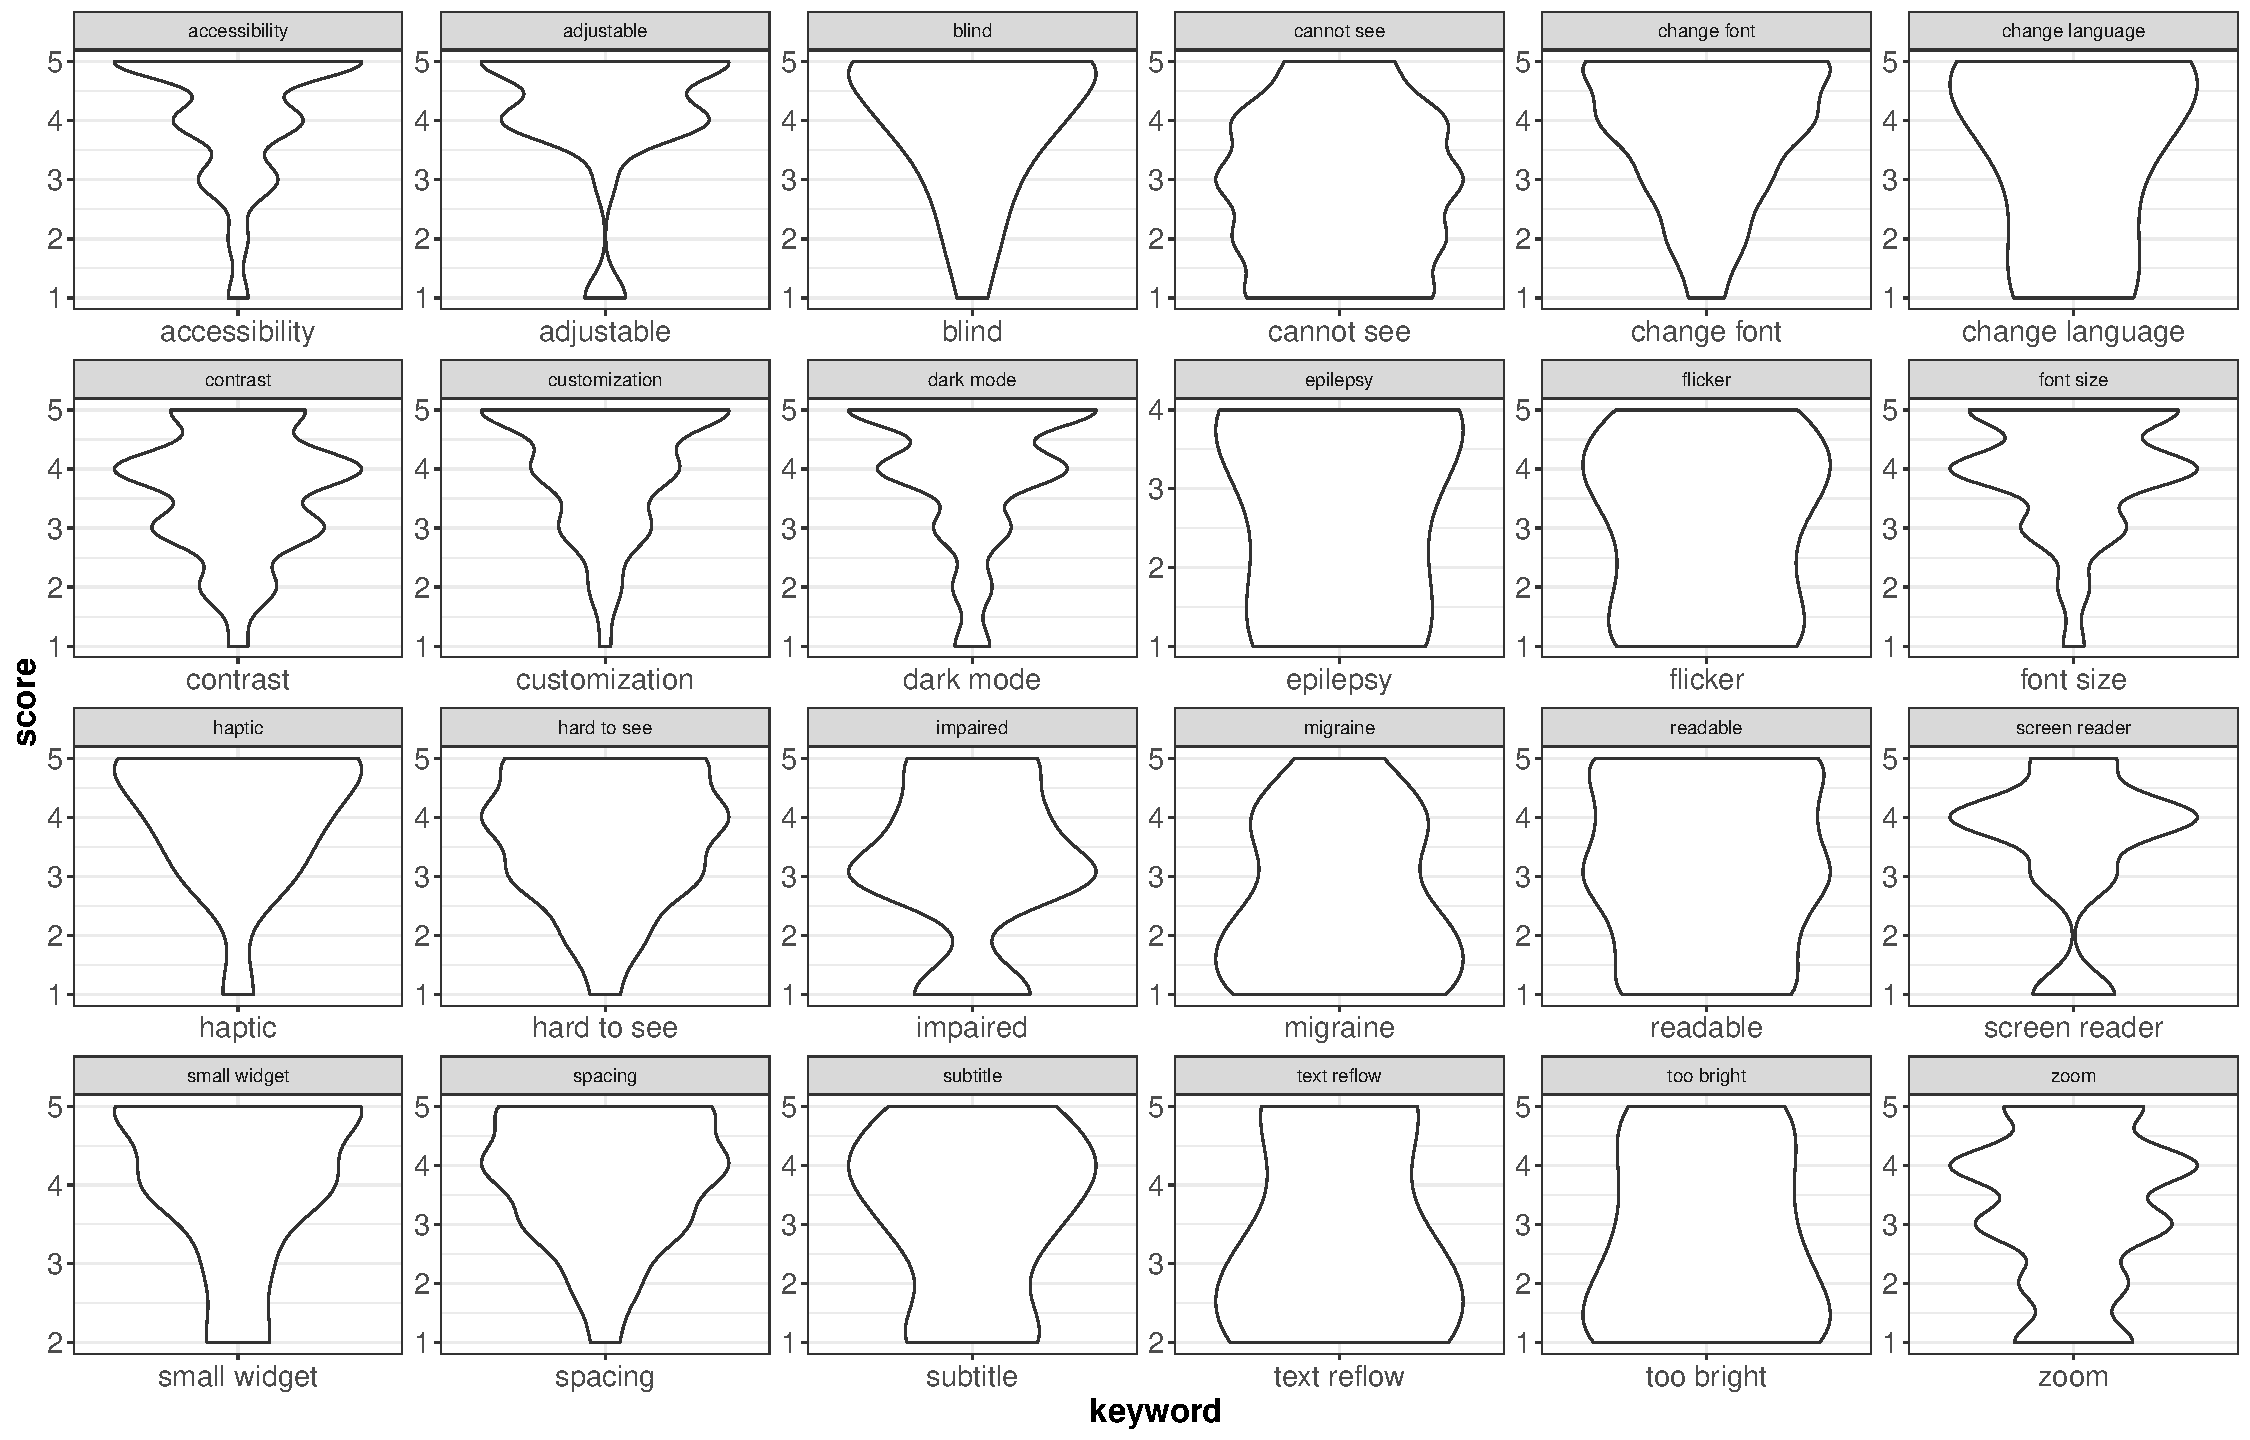
\includegraphics[scale=0.42]{imagens/keywords-scores.pdf}
\caption{Scores associated with the reviews that present a particular keyword}
\label{fig:scoreskeys}
\end{figure*}

\autoref{fig:scoreskeys} shows violin plots of the scores given by users to accessibility reviews that contain specific keywords. We do not show scores for all keywords due to space limitations. 
For some keywords, the scores are concentrated on the upper score level. This is the case of ``accessibility'', ``blind'', ``change font'', ``dark mode'', ``customization'', ``haptic'', and so forth. 
For others, there is a significant number of reviews with lower scores, such as in ``cannot see'', ``epilepsy'', ``flicker'', ``migraine'', ``readable'', ``text reflow'', and ``too bright''. This makes sense once the issues reported on reviews associated with such keywords are real barriers faced by users. Here are some examples of reviews that contain some of these keywords:
\begin{itemize}
 \item \textit{``Very little contrast. Bad for old eyes.''}
 \item \textit{``Wish it also handled older open doc formats - and that it would reflow text on zoom''}
 \item \textit{`` The flashing backgrounds could trigger an epilepsy and migraine''}
 \item \textit{``It's ok but the editing icons come up in white over the image.. which obviously means if you have a white image you cannot see them. Seriously - how could a developer get something so obvious that wrong? ''}
 \item \textit{`` Widget Text color is black. Unreadable''}
 \item \textit{``Too bright now on this update now. Can you option to inverted color? (black instead of white). Going to have to uninstall. Sorry.''}  
\end{itemize}

%Analyse reviews with the lowest scores (score == 1)


